

\tikzset{every picture/.style={line width=0.75pt}} %set default line width to 0.75pt        

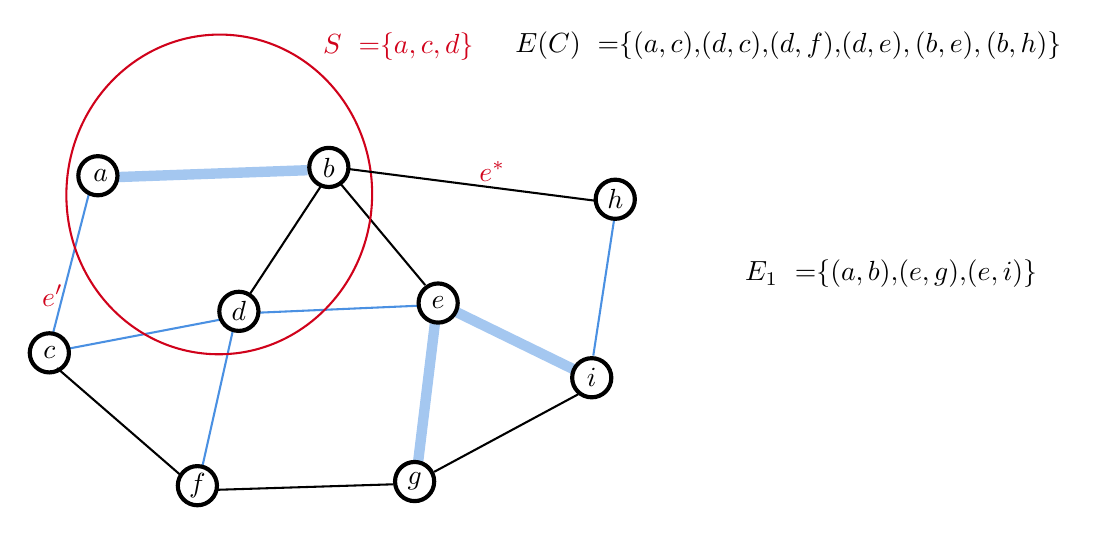
\begin{tikzpicture}[x=0.5pt,y=0.5pt,yscale=-1,xscale=1]
%uncomment if require: \path (0,388); %set diagram left start at 0, and has height of 388

%Straight Lines [id:da6859712806144006] 
\draw [color={rgb, 255:red, 0; green, 0; blue, 0 }  ,draw opacity=1 ][line width=0.75]    (232,125) -- (293,198) ;
%Straight Lines [id:da43828905709564314] 
\draw [color={rgb, 255:red, 0; green, 0; blue, 0 }  ,draw opacity=1 ][line width=0.75]    (142,346) -- (270,342) ;
%Straight Lines [id:da6385368954330931] 
\draw [color={rgb, 255:red, 0; green, 0; blue, 0 }  ,draw opacity=1 ][line width=0.75]    (27,258) -- (117,336) ;
%Straight Lines [id:da061278223687582845] 
\draw [color={rgb, 255:red, 74; green, 144; blue, 226 }  ,draw opacity=1 ][line width=0.75]    (35,244) -- (145,223) ;
%Straight Lines [id:da125058897644165] 
\draw [color={rgb, 255:red, 74; green, 144; blue, 226 }  ,draw opacity=1 ][line width=0.75]    (50,132) -- (24,233) ;
%Straight Lines [id:da7561477389708726] 
\draw [color={rgb, 255:red, 74; green, 144; blue, 226 }  ,draw opacity=0.5 ][line width=3.75]    (70,120) -- (208,115) ;
%Straight Lines [id:da8045438090716241] 
\draw [color={rgb, 255:red, 0; green, 0; blue, 0 }  ,draw opacity=1 ][line width=0.75]    (218,126) -- (166,205) ;
%Straight Lines [id:da7384444755679203] 
\draw [color={rgb, 255:red, 74; green, 144; blue, 226 }  ,draw opacity=1 ][line width=0.75]    (154,231) -- (132,329) ;
%Straight Lines [id:da7781378597799559] 
\draw [color={rgb, 255:red, 74; green, 144; blue, 226 }  ,draw opacity=0.5 ][line width=3.75]    (300,226) -- (288,325) ;
%Straight Lines [id:da6283012441188964] 
\draw [color={rgb, 255:red, 74; green, 144; blue, 226 }  ,draw opacity=1 ][line width=0.75]    (287,213) -- (172,218) ;
%Shape: Ellipse [id:dp6140347486409217] 
\draw  [color={rgb, 255:red, 208; green, 2; blue, 27 }  ,draw opacity=1 ] (33.78,128.41) .. controls (36.15,64.65) and (87.51,14.79) .. (148.48,17.06) .. controls (209.45,19.33) and (256.96,72.86) .. (254.59,136.62) .. controls (252.22,200.38) and (200.87,250.23) .. (139.89,247.96) .. controls (78.92,245.7) and (31.41,192.17) .. (33.78,128.41) -- cycle ;
%Straight Lines [id:da9156710101046748] 
\draw [color={rgb, 255:red, 0; green, 0; blue, 0 }  ,draw opacity=1 ][line width=0.75]    (236.5,114) -- (415.5,137) ;
%Straight Lines [id:da2929261017329614] 
\draw [color={rgb, 255:red, 74; green, 144; blue, 226 }  ,draw opacity=1 ][line width=0.75]    (414.5,249) -- (429.5,151) ;
%Straight Lines [id:da47669871576284994] 
\draw [color={rgb, 255:red, 74; green, 144; blue, 226 }  ,draw opacity=0.5 ][line width=3.75]    (314.5,217) -- (400.5,259) ;
%Straight Lines [id:da851369784287132] 
\draw [color={rgb, 255:red, 0; green, 0; blue, 0 }  ,draw opacity=1 ][line width=0.75]    (299.5,333) -- (403.5,277) ;

% Text Node
\draw  [line width=1.5]   (302.38, 211) circle [x radius= 14.15, y radius= 14.15]   ;
\draw (302.38,211) node   [align=left] {$\displaystyle e$};
% Text Node
\draw  [line width=1.5]   (56.48, 119) circle [x radius= 14.15, y radius= 14.15]   ;
\draw (50.98,119) node [anchor=west] [inner sep=0.75pt]   [align=left] {$\displaystyle a$};
% Text Node
\draw  [line width=1.5]   (223.38, 113) circle [x radius= 14.15, y radius= 14.15]   ;
\draw (223.38,113) node   [align=left] {$\displaystyle b$};
% Text Node
\draw  [line width=1.5]   (21.38, 247) circle [x radius= 14.15, y radius= 14.15]   ;
\draw (21.38,247) node   [align=left] {$\displaystyle c$};
% Text Node
\draw  [line width=1.5]   (158.38, 217) circle [x radius= 14.15, y radius= 14.15]   ;
\draw (158.38,217) node   [align=left] {$\displaystyle d$};
% Text Node
\draw  [line width=1.5]   (128.38, 343) circle [x radius= 14.15, y radius= 14.15]   ;
\draw (128.38,343) node   [align=left] {$\displaystyle f$};
% Text Node
\draw  [line width=1.5]   (285.38, 340) circle [x radius= 14.15, y radius= 14.15]   ;
\draw (285.38,340) node   [align=left] {$\displaystyle g$};
% Text Node
\draw (217,13.5) node [anchor=north west][inner sep=0.75pt]   [align=left] {$\displaystyle \textcolor[rgb]{0.82,0.01,0.11}{S\ =}\textcolor[rgb]{0.82,0.01,0.11}{\{}\textcolor[rgb]{0.82,0.01,0.11}{a,c,d}\textcolor[rgb]{0.82,0.01,0.11}{\}}\textcolor[rgb]{0.82,0.01,0.11}{\ }$};
% Text Node
\draw (522,177.75) node [anchor=north west][inner sep=0.75pt]   [align=left] {$\displaystyle \textcolor[rgb]{0,0,0}{E_{1} \ =}\textcolor[rgb]{0,0,0}{\{}\textcolor[rgb]{0,0,0}{(}\textcolor[rgb]{0,0,0}{a,b}\textcolor[rgb]{0,0,0}{)}\textcolor[rgb]{0,0,0}{,}\textcolor[rgb]{0,0,0}{(}\textcolor[rgb]{0,0,0}{e,g}\textcolor[rgb]{0,0,0}{)}\textcolor[rgb]{0,0,0}{,}\textcolor[rgb]{0,0,0}{(}\textcolor[rgb]{0,0,0}{e,i}\textcolor[rgb]{0,0,0}{)}\textcolor[rgb]{0,0,0}{\}}\textcolor[rgb]{0,0,0}{\ }$};
% Text Node
\draw  [line width=1.5]   (430.38, 136) circle [x radius= 14.15, y radius= 14.15]   ;
\draw (430.38,136) node   [align=left] {$\displaystyle h$};
% Text Node
\draw  [line width=1.5]   (413.38, 265) circle [x radius= 14.15, y radius= 14.15]   ;
\draw (413.38,265) node   [align=left] {$\displaystyle i$};
% Text Node
\draw (356,12.75) node [anchor=north west][inner sep=0.75pt]   [align=left] {$\displaystyle \textcolor[rgb]{0,0,0}{E( C) \ =}\textcolor[rgb]{0,0,0}{\{}\textcolor[rgb]{0,0,0}{(}\textcolor[rgb]{0,0,0}{a,c}\textcolor[rgb]{0,0,0}{)}\textcolor[rgb]{0,0,0}{,}\textcolor[rgb]{0,0,0}{(}\textcolor[rgb]{0,0,0}{d,c}\textcolor[rgb]{0,0,0}{)}\textcolor[rgb]{0,0,0}{,}\textcolor[rgb]{0,0,0}{(}\textcolor[rgb]{0,0,0}{d,f}\textcolor[rgb]{0,0,0}{) ,}\textcolor[rgb]{0,0,0}{( d,e) ,( b,e) ,( b,h)\}}\textcolor[rgb]{0,0,0}{\ }$};
% Text Node
\draw (330,106.5) node [anchor=north west][inner sep=0.75pt]   [align=left] {$\displaystyle \textcolor[rgb]{0.82,0.01,0.11}{e}\textcolor[rgb]{0.82,0.01,0.11}{^{*} \ }$};
% Text Node
\draw (14,195.5) node [anchor=north west][inner sep=0.75pt]   [align=left] {$\displaystyle \textcolor[rgb]{0.82,0.01,0.11}{e'\ }$};


\end{tikzpicture}

